% =============================================================================
% Lecture 04: Stationarity and ARIMA
% BSAD 8310: Business Forecasting
% University of Nebraska at Omaha
% =============================================================================

\documentclass[aspectratio=169, 11pt]{beamer}

% =============================================================================
% header.tex — BSAD 8310: Business Forecasting
% University of Nebraska at Omaha
% Beamer theme: UNO-branded, clean, professional
% =============================================================================

% ----------------------------- BEAMER THEME ----------------------------------
\usetheme{default}
\useinnertheme{rectangles}

% ----------------------------- UNO COLOR PALETTE -----------------------------
\definecolor{unoblue}{HTML}{005CA9}
\definecolor{unored}{HTML}{E41C38}
\definecolor{unogray}{HTML}{525252}
\definecolor{unogreen}{HTML}{15803d}
\definecolor{unolightblue}{HTML}{E8F0FA}
\definecolor{unolightred}{HTML}{FDECEA}
\definecolor{unolightgreen}{HTML}{F0FAF4}
\definecolor{unowhite}{HTML}{FFFFFF}

% Apply UNO colors to Beamer structure
\setbeamercolor{structure}{fg=unoblue}
\setbeamercolor{palette primary}{bg=unoblue, fg=white}
\setbeamercolor{palette secondary}{bg=unoblue!80!black, fg=white}
\setbeamercolor{palette tertiary}{bg=unoblue!60!black, fg=white}
\setbeamercolor{frametitle}{bg=unoblue, fg=white}
\setbeamercolor{frametitle right}{bg=unoblue!80!black}
\setbeamercolor{title}{fg=unoblue}
\setbeamercolor{subtitle}{fg=unogray}
\setbeamercolor{author in head/foot}{bg=unoblue, fg=white}
\setbeamercolor{title in head/foot}{bg=unoblue!80, fg=white}
\setbeamercolor{date in head/foot}{bg=unoblue!60, fg=white}
\setbeamercolor{page number in head/foot}{bg=unoblue!60, fg=white}
\setbeamercolor{block title}{bg=unoblue, fg=white}
\setbeamercolor{block body}{bg=unolightblue}
\setbeamercolor{block title alerted}{bg=unored, fg=white}
\setbeamercolor{block body alerted}{bg=unolightred}
\setbeamercolor{block title example}{bg=unogreen, fg=white}
\setbeamercolor{block body example}{bg=unolightgreen}
\setbeamercolor{itemize item}{fg=unoblue}
\setbeamercolor{itemize subitem}{fg=unored}
\setbeamercolor{enumerate item}{fg=unoblue}
\setbeamercolor{enumerate subitem}{fg=unored}
\setbeamercolor{alerted text}{fg=unored}

% ----------------------------- FONTS -----------------------------------------
\usefonttheme{professionalfonts}
\usefonttheme[onlymath]{serif}       % serif math; sans-serif text
\setbeamerfont{frametitle}{size=\large, series=\bfseries}
\setbeamerfont{title}{size=\LARGE, series=\bfseries}
\setbeamerfont{subtitle}{size=\large}
\setbeamerfont{block title}{size=\normalsize, series=\bfseries}
\setbeamerfont{footline}{size=\tiny}

% ----------------------------- LAYOUT ----------------------------------------
\setbeamersize{text margin left=0.5cm, text margin right=0.5cm}
\setbeamertemplate{navigation symbols}{}   % remove navigation buttons
\setbeamertemplate{itemize items}[circle]
\setbeamertemplate{enumerate items}[default]

% Custom footline: [Course] [Title] [Page/Total]
\setbeamertemplate{footline}{%
  \leavevmode%
  \hbox{%
    \begin{beamercolorbox}[wd=.33\paperwidth, ht=2.5ex, dp=1ex, left, leftskip=4pt]
      {author in head/foot}%
      \usebeamerfont{author in head/foot}\insertshortauthor
    \end{beamercolorbox}%
    \begin{beamercolorbox}[wd=.34\paperwidth, ht=2.5ex, dp=1ex, center]
      {title in head/foot}%
      \usebeamerfont{title in head/foot}\insertshorttitle
    \end{beamercolorbox}%
    \begin{beamercolorbox}[wd=.33\paperwidth, ht=2.5ex, dp=1ex, right, rightskip=4pt]
      {date in head/foot}%
      \usebeamerfont{date in head/foot}%
      \insertframenumber{} / \inserttotalframenumber
    \end{beamercolorbox}%
  }%
  \vskip0pt%
}

% Frametitle with thin accent line
\setbeamertemplate{frametitle}{%
  \vskip0.1cm
  \insertframetitle
  \vskip0.05cm
  \color{unored}\rule{\textwidth}{0.5pt}
}

% Title page
\setbeamertemplate{title page}{%
  \vfill
  \begin{center}
    {\color{unoblue}\rule{\textwidth}{2pt}}\\[0.3cm]
    {\usebeamerfont{title}\usebeamercolor[fg]{title}\inserttitle}\\[0.2cm]
    {\usebeamerfont{subtitle}\usebeamercolor[fg]{subtitle}\insertsubtitle}\\[0.3cm]
    {\color{unored}\rule{\textwidth}{0.5pt}}\\[0.4cm]
    {\small\insertauthor}\\[0.1cm]
    {\small\insertinstitute}\\[0.1cm]
    {\small\insertdate}
  \end{center}
  \vfill
}

% ----------------------------- PACKAGES --------------------------------------

% Math
\usepackage{amsmath}
\usepackage{amssymb}
\usepackage{mathtools}
\usepackage{bm}                    % bold math symbols

% Graphics & color
\usepackage{graphicx}
\usepackage{xcolor}
\usepackage{tikz}
\usetikzlibrary{arrows.meta, positioning, shapes, fit, backgrounds, calc}
\usepackage{pgfplots}
\pgfplotsset{compat=1.18}

% Tables
\usepackage{booktabs}
\usepackage{array}
\usepackage{multirow}
\usepackage{tabularx}

% Typography
\usepackage{microtype}
\usepackage{url}
\usepackage{hyperref}
\hypersetup{colorlinks=true, linkcolor=unoblue, urlcolor=unoblue, citecolor=unogray}

% Code listings (no shell-escape required)
\usepackage{listings}
\lstset{
  language=Python,
  basicstyle=\ttfamily\footnotesize,
  keywordstyle=\color{unoblue}\bfseries,
  stringstyle=\color{unogreen},
  commentstyle=\color{unogray}\itshape,
  numberstyle=\tiny\color{unogray},
  breaklines=true,
  showstringspaces=false,
  frame=single,
  rulecolor=\color{unogray!40},
  backgroundcolor=\color{unogray!5},
  xleftmargin=0.5em,
  xrightmargin=0.5em,
}

% Bibliography
\usepackage[backend=bibtex, style=authoryear, maxcitenames=2]{biblatex}
\addbibresource{../Bibliography_base.bib}

% Colored text helpers
\usepackage{tcolorbox}
\tcbuselibrary{skins, breakable, listingsutf8}

% ----------------------------- CUSTOM ENVIRONMENTS ---------------------------

% keybox: UNO-blue background — for key results, formulas, takeaways
\newtcolorbox{keybox}{
  enhanced,
  colback=unoblue,
  colframe=unoblue!80!black,
  coltitle=white,
  coltext=white,
  fonttitle=\bfseries,
  boxrule=0pt,
  arc=3pt,
  left=4pt, right=4pt, top=3pt, bottom=3pt,
}

% definitionbox: blue left-rule with title — for formal definitions
\newtcolorbox{definitionbox}[1]{
  enhanced,
  title={#1},
  colback=unolightblue,
  colframe=unoblue,
  coltitle=unoblue,
  fonttitle=\bfseries,
  boxrule=0pt,
  leftrule=3pt,
  arc=0pt,
  left=4pt, right=4pt, top=3pt, bottom=3pt,
}

% warningbox: red-accent — for pitfalls, assumption violations, common errors
\newtcolorbox{warningbox}{
  enhanced,
  colback=unolightred,
  colframe=unored,
  coltitle=white,
  fonttitle=\bfseries,
  boxrule=0pt,
  leftrule=3pt,
  arc=0pt,
  left=4pt, right=4pt, top=3pt, bottom=3pt,
}

% examplebox: green-accent with title — for worked examples, business applications
\newtcolorbox{examplebox}[1]{
  enhanced,
  title={#1},
  colback=unolightgreen,
  colframe=unogreen,
  coltitle=unogreen,
  fonttitle=\bfseries,
  boxrule=0pt,
  leftrule=3pt,
  arc=0pt,
  left=4pt, right=4pt, top=3pt, bottom=3pt,
}

% ----------------------------- MATH SHORTCUTS --------------------------------
\newcommand{\E}{\mathbb{E}}
\newcommand{\Var}{\operatorname{Var}}
\newcommand{\Cov}{\operatorname{Cov}}
\newcommand{\Corr}{\operatorname{Corr}}
\newcommand{\MSE}{\operatorname{MSE}}
\newcommand{\RMSE}{\operatorname{RMSE}}
\newcommand{\MAE}{\operatorname{MAE}}
\newcommand{\MASE}{\operatorname{MASE}}
\newcommand{\yhat}{\hat{y}}
\newcommand{\bhat}{\hat{\beta}}
\newcommand{\eps}{\varepsilon}
\newcommand{\given}{\,|\,}

% ----------------------------- SLIDE HELPERS ---------------------------------
% Section title slide (call at start of each section)
\newcommand{\sectionslide}[2]{%
  \begin{frame}
    \vfill
    \begin{center}
      {\color{unoblue}\rule{0.6\textwidth}{2pt}}\\[0.4cm]
      {\Large\bfseries\color{unoblue} #1}\\[0.2cm]
      {\normalsize\color{unogray} #2}\\[0.4cm]
      {\color{unored}\rule{0.6\textwidth}{1pt}}
    \end{center}
    \vfill
  \end{frame}
}

% Muted text
\newcommand{\muted}[1]{{\color{unogray}#1}}

% Key term
\newcommand{\key}[1]{{\color{unoblue}\textbf{#1}}}

% Positive / negative annotations
\newcommand{\pos}[1]{{\color{unogreen}#1}}
\newcommand{\negc}[1]{{\color{unored}#1}}


% ---- Lecture metadata --------------------------------------------------------
\title{Stationarity and ARIMA}
\subtitle{BSAD 8310: Business Forecasting --- Lecture 4}
\author{Department of Economics}
\institute{University of Nebraska at Omaha}
\date{Spring 2026}

% =============================================================================
\begin{document}
% =============================================================================

\begin{frame}
  \titlepage
\end{frame}

% --- Outline -----------------------------------------------------------------
\begin{frame}{Lecture 4: Outline}
  \tableofcontents
\end{frame}

% =============================================================================
\section{Stationarity}
% =============================================================================

\sectionslide{Stationarity}{%
  All classical forecasting models implicitly assume a stable data-generating process.}

% --- Slide: Weak stationarity definition -------------------------------------
\begin{frame}{Weak (Covariance) Stationarity}
  \begin{definitionbox}{Weak Stationarity}
    A time series $\{y_t\}$ is \textbf{weakly stationary} if:
    \begin{enumerate}\small
      \item $\E[y_t] = \mu$ \quad (constant mean)
      \item $\Var(y_t) = \sigma^2 < \infty$ \quad (constant, finite variance)
      \item $\Cov(y_t, y_{t-k}) = \gamma_k$ depends only on lag $k$,
            not on $t$
    \end{enumerate}
  \end{definitionbox}
  \vspace{0.1cm}
  \textbf{Why it matters for forecasting:}
  \begin{itemize}\small
    \item If $\E[y_t]$ changes over time, no single mean is forecastable
    \item If $\Var(y_t) \to \infty$, prediction intervals become unbounded
    \item Stationarity is what makes past patterns informative about the future
  \end{itemize}
  \muted{\footnotesize\itshape
    Socratic: if $y_t = t + \varepsilon_t$ (linear trend plus white noise),
    which stationarity condition does it violate?}
\end{frame}

% --- Slide: Stationary vs. non-stationary visual ------------------------------
\begin{frame}{Stationary vs.\ Non-Stationary: A Visual Comparison}
  \begin{columns}[T]
    \column{0.48\textwidth}
      \textbf{AR(1)-like series, $\phi_1 = 0.7$ (simulated):}
      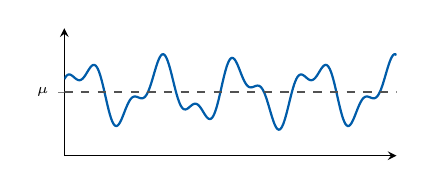
\begin{tikzpicture}
        \begin{axis}[
          width=5.8cm, height=3.2cm,
          xmin=0, xmax=30, ymin=-3, ymax=3,
          xtick=\empty, ytick={0},
          yticklabels={$\mu$},
          axis lines=left,
          tick label style={font=\tiny},
        ]
          \addplot[color=unoblue, thick, domain=0:30, samples=300]
            {1.2*sin(deg(0.9*x)) + 0.6*cos(deg(2.1*x))};
          \addplot[color=unogray, dashed, domain=0:30] {0};
        \end{axis}
      \end{tikzpicture}\\[2pt]
      \muted{\footnotesize Fluctuates around $\mu$; bounded variance.}
    \column{0.48\textwidth}
      \textbf{Random-walk-like series, $\phi_1 = 1$ (simulated):}
      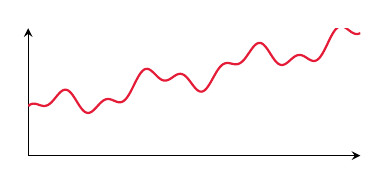
\begin{tikzpicture}
        \begin{axis}[
          width=5.8cm, height=3.2cm,
          xmin=0, xmax=30, ymin=-3, ymax=6,
          xtick=\empty, ytick=\empty,
          axis lines=left,
          tick label style={font=\tiny},
        ]
          \addplot[color=unored, thick, domain=0:30, samples=300]
            {0.18*x + 0.8*sin(deg(0.7*x)) + 0.5*cos(deg(1.8*x))};
        \end{axis}
      \end{tikzpicture}\\[2pt]
      \muted{\footnotesize Drifts without bound; variance grows with $t$.}
  \end{columns}
  \begin{keybox}
    ETS and AR models require stationarity (or achieve it via trend/seasonal
    components). ARIMA handles non-stationarity through \textbf{differencing}.
  \end{keybox}
\end{frame}

% =============================================================================
\section{Unit Roots and Differencing}
% =============================================================================

\sectionslide{Unit Roots and Differencing}{%
  A random walk has a unit root --- shocks accumulate permanently.}

% --- Slide: The unit root -----------------------------------------------------
\begin{frame}{The Unit Root}
  Consider the AR(1) model: $y_t = \phi_1\,y_{t-1} + \varepsilon_t$
  \begin{center}
    {\small
    \begin{tabular}{lll}
      \toprule
      \textbf{Condition} & \textbf{Behavior} & \textbf{Process} \\
      \midrule
      $|\phi_1| < 1$ & Shock decays geometrically & Stationary AR(1) \\
      $\phi_1 = 1$   & Shock persists permanently & Random walk (unit root) \\
      $|\phi_1| > 1$ & Explosion & Explosive (not forecastable) \\
      \bottomrule
    \end{tabular}
    }
  \end{center}
  \vspace{0.1cm}
  \textbf{Random walk expanded:} $y_T = y_0 + \sum_{t=1}^{T}\varepsilon_t$
  \begin{warningbox}
    {\small With a unit root, the \textbf{effect of every past shock is permanent}.
    The na\"{i}ve forecast $\hat{y}_{T+h|T} = y_T$ is optimal for a pure
    random walk --- and the forecast variance grows as $h\sigma^2$.}
  \end{warningbox}
\end{frame}

% --- Slide: ADF test ----------------------------------------------------------
\begin{frame}{Testing for a Unit Root: The ADF Test}
  Rewrite the AR(1) as a regression:
  \[
    \Delta y_t \;=\; \delta\, y_{t-1} \;+\; \varepsilon_t,
    \qquad \delta = \phi_1 - 1
  \]
  \begin{definitionbox}{Augmented Dickey-Fuller (ADF) Test}
    {\small
    $H_0: \delta = 0$ \quad (unit root --- non-stationary)\\[2pt]
    $H_1: \delta < 0$ \quad (stationary)\\[2pt]
    Test statistic: $\tau = \hat{\delta}/\mathrm{SE}(\hat{\delta})$
    follows a non-standard distribution; critical values from
    \textcite{DickeyFuller1979}.}
  \end{definitionbox}
  \textbf{Augmentation:} include $\Delta y_{t-1}, \ldots, \Delta y_{t-p}$
  lags to remove residual autocorrelation. Also include a constant and/or
  linear trend as appropriate.
  \muted{\footnotesize\itshape
    Socratic: the ADF statistic does not follow a standard $t$-distribution
    even in large samples. What does this mean for using standard regression
    $p$-values to test for a unit root?}
\end{frame}

% --- Slide: Differencing ------------------------------------------------------
\begin{frame}{Differencing: Removing Non-Stationarity}
  \textbf{First difference} removes a stochastic trend (unit root):
  \[
    \Delta y_t \;=\; y_t - y_{t-1} \;=\; (1-B)\,y_t
  \]
  where $B$ is the \textbf{backshift operator} ($By_t = y_{t-1}$).
  \begin{columns}[T]
    \column{0.50\textwidth}
      \textbf{Seasonal difference} removes seasonal non-stationarity:
      \[
        \Delta_m y_t = y_t - y_{t-m} = (1-B^m)\,y_t
      \]
      For monthly data: $\Delta_{12} y_t = y_t - y_{t-12}$.
    \column{0.46\textwidth}
      \begin{keybox}
        {\small
        $d=0$: already stationary\\
        $d=1$: one first difference\\
        $d=2$: rarely needed\\
        $D=1$: one seasonal difference
        }
      \end{keybox}
  \end{columns}
  \vspace{0.1cm}
  \begin{warningbox}
    \textbf{Over-differencing} induces negative autocorrelation.
    Re-apply ADF/KPSS after differencing: if $\Delta y_t$ is stationary,
    stop at $d=1$. Over-differencing introduces MA unit roots.
  \end{warningbox}
\end{frame}

% --- Slide: KPSS as complement ------------------------------------------------
\begin{frame}{Complementary Test: KPSS}
  The ADF and KPSS tests address \emph{opposite} null hypotheses.
  \muted{\footnotesize (KPSS: Kwiatkowski--Phillips--Schmidt--Shin)}
  \begin{center}
    {\small
    \begin{tabular}{lll}
      \toprule
      \textbf{Test} & \textbf{$H_0$} & \textbf{$H_1$} \\
      \midrule
      ADF \parencite{DickeyFuller1979}    & Unit root (non-stationary) & Stationary \\
      KPSS \parencite{Kwiatkowski1992}    & Stationary                 & Unit root \\
      \bottomrule
    \end{tabular}
    }
  \end{center}
  \vspace{0.1cm}
  \textbf{Practical workflow:}
  \begin{enumerate}\small
    \item ADF: fail to reject $\Rightarrow$ evidence of unit root
    \item KPSS: reject $\Rightarrow$ evidence against stationarity
    \item If both agree $\Rightarrow$ high confidence; if conflicting $\Rightarrow$
          inspect ACF and apply domain knowledge
  \end{enumerate}
  \muted{\footnotesize\itshape
    Automatic order selection (\texttt{pmdarima.auto\_arima}) runs ADF internally
    to determine $d$ before fitting ARIMA.}
\end{frame}

% =============================================================================
\section{ACF and PACF}
% =============================================================================

\sectionslide{ACF and PACF}{%
  The autocorrelation function is the fingerprint of a time series.}

% --- Slide: ACF ---------------------------------------------------------------
\begin{frame}{The Autocorrelation Function (ACF)}
  \begin{definitionbox}{Autocorrelation Function}
    The \textbf{lag-$k$ autocorrelation} of a stationary series:
    \[
      \rho_k \;=\; \frac{\Cov(y_t,\,y_{t-k})}{\Var(y_t)}
             \;=\; \frac{\gamma_k}{\gamma_0},
      \qquad k = 1, 2, \ldots
    \]
    Estimated by $\hat{\rho}_k$; 95\% confidence bounds $\approx \pm 1.96/\sqrt{T}$.
  \end{definitionbox}
  \textbf{Theoretical ACF for AR(1):} $\rho_k = \phi_1^k$ \quad (geometric decay):
  \begin{center}
  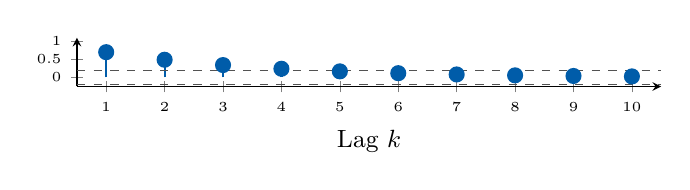
\begin{tikzpicture}
    \begin{axis}[
      width=9cm, height=2.2cm,
      xlabel={Lag $k$},
      xmin=0.5, xmax=10.5, ymin=-0.25, ymax=1.1,
      xtick={1,2,...,10}, ytick={0,0.5,1},
      axis lines=left,
      tick label style={font=\tiny},
      label style={font=\small},
      yticklabels={0,0.5,1},
    ]
      \addplot[ycomb, color=unoblue, thick, mark=*, mark size=2.5pt,
               samples at={1,2,...,10}] {0.7^x};
      \addplot[dashed, color=unogray, domain=0.5:10.5] {0.196};
      \addplot[dashed, color=unogray, domain=0.5:10.5] {-0.196};
    \end{axis}
  \end{tikzpicture}
  \end{center}
  \muted{\footnotesize\itshape
    Dashed lines: $\pm 1.96/\sqrt{T}$ bounds ($T=100$).
    Bars outside bounds are statistically significant.}
\end{frame}

% --- Slide: PACF ---------------------------------------------------------------
\begin{frame}{The Partial Autocorrelation Function (PACF)}
  \begin{columns}[T]
    \column{0.52\textwidth}
      \begin{definitionbox}{Partial Autocorrelation}
        The \textbf{lag-$k$ PACF} $\phi_{kk}$ is the correlation between
        $y_t$ and $y_{t-k}$ \emph{after removing} the linear effects
        of $y_{t-1}, \ldots, y_{t-k+1}$.
      \end{definitionbox}
      \vspace{0.1cm}
      \textbf{For model identification:}
      \begin{itemize}\small
        \item AR($p$): $\phi_{kk} = 0$ for $k > p$
              $\Rightarrow$ PACF \textbf{cuts off} after lag $p$
        \item MA($q$): $\phi_{kk} \to 0$ geometrically as $k \to \infty$
              $\Rightarrow$ PACF \textbf{tails off}
      \end{itemize}
    \column{0.46\textwidth}
      \textbf{Theoretical PACF for AR(2):}
      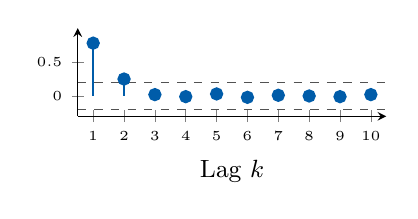
\begin{tikzpicture}
        \begin{axis}[
          width=5.5cm, height=2.7cm,
          xlabel={Lag $k$},
          xmin=0.5, xmax=10.5, ymin=-0.3, ymax=1.0,
          xtick={1,2,...,10}, ytick={0,0.5},
          axis lines=left,
          tick label style={font=\tiny},
          label style={font=\small},
        ]
          \addplot[ycomb, color=unoblue, thick, mark=*, mark size=2pt]
            coordinates {(1,0.78)(2,0.25)(3,0.02)(4,-0.01)
                         (5,0.03)(6,-0.02)(7,0.01)(8,0.00)
                         (9,-0.01)(10,0.02)};
          \addplot[dashed, color=unogray, domain=0.5:10.5] {0.196};
          \addplot[dashed, color=unogray, domain=0.5:10.5] {-0.196};
        \end{axis}
      \end{tikzpicture}\\[-3pt]
      \muted{\footnotesize\itshape Cuts off after lag 2: AR(2) signature.}
  \end{columns}
  \begin{keybox}
    {\small ACF identifies MA order~($q$); PACF identifies AR order~($p$).
    Together they form the Box-Jenkins identification toolkit.}
  \end{keybox}
\end{frame}

% --- Slide: Pattern recognition table -----------------------------------------
\begin{frame}{ACF/PACF Pattern Recognition}
  \begin{center}
    \begin{tabular}{llll}
      \toprule
      \textbf{Model} & \textbf{ACF} & \textbf{PACF} & $\boldsymbol{d}$ \\
      \midrule
      White noise    & No significant spikes & No significant spikes & 0 \\
      AR($p$)        & Tails off (decays) & \pos{Cuts off after $p$} & 0 \\
      MA($q$)        & \pos{Cuts off after $q$} & Tails off (decays) & 0 \\
      ARMA($p$,$q$)  & Tails off & Tails off & 0 \\
      Random walk    & Decays very slowly & Large spike at lag 1 & 1 \\
      \bottomrule
    \end{tabular}
  \end{center}
  \vspace{0.1cm}
  \begin{warningbox}
    Always unit-root test and difference \emph{before} reading ACF/PACF.
    The ACF/PACF of a non-stationary series are not interpretable.
  \end{warningbox}
\end{frame}

% =============================================================================
\section{The ARIMA Model}
% =============================================================================

\sectionslide{The ARIMA Model}{%
  ARIMA = differencing to achieve stationarity $+$ ARMA on the result.}

% --- Slide: ARMA(p,q) ---------------------------------------------------------
\begin{frame}{From AR to ARMA($p$,$q$)}
  \textbf{AR($p$):} $y_t = c + \phi_1 y_{t-1} + \cdots + \phi_p y_{t-p} + \varepsilon_t$

  \textbf{MA($q$):} $y_t = c + \varepsilon_t + \theta_1\varepsilon_{t-1}
                    + \cdots + \theta_q\varepsilon_{t-q}$
  \muted{\footnotesize\itshape MA terms arise naturally from aggregation and averaging ---
    notably, ARIMA(0,1,1) is algebraically equivalent to SES.}

  \begin{definitionbox}{ARMA($p$,$q$) Model}
    {\small
    \[
      y_t = c + \sum_{i=1}^{p}\phi_i y_{t-i}
              + \varepsilon_t
              + \sum_{j=1}^{q}\theta_j\varepsilon_{t-j},
      \qquad \varepsilon_t \overset{iid}{\sim}\mathcal{N}(0,\sigma^2)
    \]
    MA terms capture autocorrelation in \emph{shocks}; AR terms capture
    autocorrelation in \emph{levels}.}
  \end{definitionbox}
  \begin{columns}[T]
    \column{0.48\textwidth}
      \textbf{Special cases:}\\
      ARMA($p$,0) $=$ AR($p$)\\
      ARMA(0,$q$) $=$ MA($q$)
    \column{0.48\textwidth}
      \textbf{Requirements:}\\
      Stationarity: roots of AR polynomial outside unit circle\\
      Invertibility: roots outside unit circle \muted{\footnotesize(unique MA
      representation; allows rewriting as AR($\infty$))}
  \end{columns}
\end{frame}

% --- Slide: ARIMA(p,d,q) ------------------------------------------------------
\begin{frame}{ARIMA($p$,$d$,$q$): Adding Integration}
  \begin{definitionbox}{ARIMA($p$,$d$,$q$) Model}
    Apply ARMA($p$,$q$) to the $d$-times differenced series $(1-B)^d y_t$:
    \[
      \underbrace{(1-\phi_1 B - \cdots - \phi_p B^p)}_{\text{AR polynomial}}
      \underbrace{(1-B)^d}_{\text{differencing}}
      y_t
      \;=\;
      c + \underbrace{(1+\theta_1 B + \cdots + \theta_q B^q)}_{\text{MA polynomial}}
      \varepsilon_t
    \]
  \end{definitionbox}
  \vspace{0.1cm}
  \begin{columns}[T]
    \column{0.48\textwidth}
      \textbf{Parameter meaning:}
      \begin{itemize}\small
        \item $p$: AR order (lags of $y$)
        \item $d$: degree of differencing
        \item $q$: MA order (lags of $\varepsilon$)
      \end{itemize}
    \column{0.48\textwidth}
      \textbf{Common special cases:}
      \begin{itemize}\small
        \item ARIMA(0,1,0): random walk
        \item ARIMA(1,1,0): differenced AR(1)
        \item ARIMA(0,1,1): equivalent to SES \parencite[][Ch.~9]{Hyndman2021}
      \end{itemize}
  \end{columns}
  \muted{\footnotesize\itshape
    Example (ARIMA(1,1,0), $\hat{\phi}_1=0.5$, $y_{100}=120$, $y_{99}=118$):
    $\Delta y_{100}=2 \;\Rightarrow\; \hat{y}_{101|100}=120+0.5\times 2=\mathbf{121}$}
\end{frame}

% --- Slide: Box-Jenkins methodology -------------------------------------------
\begin{frame}{Box-Jenkins Methodology \textcite{BoxJenkins2015}}
  \begin{center}
    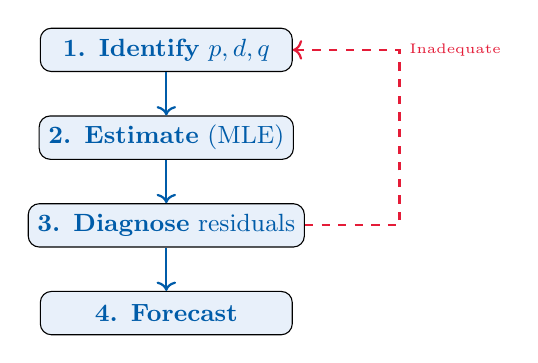
\begin{tikzpicture}[node distance=0.55cm, every node/.style={font=\small}]
      \node[draw, fill=unolightblue, rounded corners, minimum width=3.2cm,
            minimum height=0.55cm, text=unoblue] (id)
            {\textbf{1. Identify} $p,d,q$};
      \node[draw, fill=unolightblue, rounded corners, minimum width=3.2cm,
            minimum height=0.55cm, text=unoblue, below=of id] (est)
            {\textbf{2. Estimate} (MLE)};
      \node[draw, fill=unolightblue, rounded corners, minimum width=3.2cm,
            minimum height=0.55cm, text=unoblue, below=of est] (diag)
            {\textbf{3. Diagnose} residuals};
      \node[draw, fill=unolightblue, rounded corners, minimum width=3.2cm,
            minimum height=0.55cm, text=unoblue, below=of diag] (fc)
            {\textbf{4. Forecast}};
      \draw[->, thick, color=unoblue] (id) -- (est);
      \draw[->, thick, color=unoblue] (est) -- (diag);
      \draw[->, thick, color=unoblue] (diag) -- (fc);
      \draw[->, thick, color=unored, dashed]
        (diag.east) -- ++(1.2,0) |- node[right, font=\tiny,
        text=unored]{Inadequate} (id.east);
    \end{tikzpicture}
  \end{center}
  \vspace{0.1cm}
  \textbf{Step 1 (Identify):} unit root tests $\to d$; ACF/PACF $\to p,q$

  \textbf{Step 3 (Diagnose):} residual ACF should show no structure;
  Ljung-Box $H_0$: residuals are white noise \muted{\footnotesize(test at lag $L=\min(10,T/5)$;
  $p$-value $<0.05$ suggests residual autocorrelation --- re-identify)}
\end{frame}

% --- Slide: ARIMA forecast + uncertainty ------------------------------------
\begin{frame}{Forecasting with ARIMA}
  \textbf{Multi-step forecasting} uses the recursive substitution principle:
  \[
    \hat{y}_{T+h|T}
    = \hat{c} + \sum_{i=1}^{p}\hat{\phi}_i\,\hat{y}_{T+h-i|T}
                + \sum_{j=1}^{q}\hat{\theta}_j\,\hat{\varepsilon}_{T+h-j|T}
  \]
  where $\hat{y}_{T+k|T} = y_{T+k}$ for $k \leq 0$ and
  $\hat{\varepsilon}_{T+k|T} = 0$ for $k > 0$.
  \begin{keybox}
    ARIMA forecast uncertainty \textbf{grows} with horizon $h$:
    prediction interval half-width scales as $\sigma\sqrt{h}$ for ARIMA(0,1,0).
    ARIMA(0,1,1) $\equiv$ SES shares this same growing uncertainty.
  \end{keybox}
  \muted{\footnotesize\itshape
    Socratic: ARIMA(0,1,1) produces the same point forecast as SES
    with $\hat{\alpha} = 1 - \hat{\theta}_1$. Why might their
    prediction intervals still differ?}
\end{frame}

% =============================================================================
\section{Seasonal ARIMA}
% =============================================================================

\sectionslide{Seasonal ARIMA}{%
  Retail and economic data have seasonal autocorrelation at lags $m$, $2m$, $3m$,\ldots}

% --- Slide: SARIMA notation ---------------------------------------------------
\begin{frame}{SARIMA($p$,$d$,$q$)($P$,$D$,$Q$)[$m$]}
  Monthly retail data exhibit autocorrelation at lags $m, 2m, 3m, \ldots$
  beyond standard ARIMA. SARIMA extends the model with seasonal polynomials
  $\Phi_P(B^m)$ and $\Theta_Q(B^m)$:
  \begin{definitionbox}{Seasonal ARIMA (SARIMA)}
    {\small
    \[
      \underbrace{\Phi_P(B^m)}_{\text{seasonal AR}}
      \underbrace{\phi_p(B)}_{\text{AR}}
      \underbrace{(1-B^m)^D}_{\text{seas.\ diff.}}
      \underbrace{(1-B)^d}_{\text{diff.}}
      y_t
      \;=\;
      c +
      \underbrace{\Theta_Q(B^m)}_{\text{seasonal MA}}
      \underbrace{\theta_q(B)}_{\text{MA}}
      \varepsilon_t
    \]
    }
  \end{definitionbox}
  \begin{columns}[T]
    \column{0.52\textwidth}
      \textbf{Parameters:}
      \begin{itemize}\small
        \item $(p,d,q)$: non-seasonal orders
        \item $(P,D,Q)$: seasonal orders at period $m$
        \item $m=12$ for monthly; $m=4$ for quarterly
      \end{itemize}
    \column{0.44\textwidth}
      \begin{examplebox}{RSXFS retail sales}
        {\small SARIMA(1,1,1)(0,1,1)[12]
        is a common starting point for monthly retail series.}
      \end{examplebox}
  \end{columns}
\end{frame}

% --- Slide: Auto-ARIMA --------------------------------------------------------
\begin{frame}{Automatic ARIMA Selection}
  Manual identification via ACF/PACF is time-consuming and subjective.
  \textbf{Auto-ARIMA} automates the process:
  \begin{enumerate}\small
    \item Apply unit-root tests to select $d$ (and $D$)
    \item Search over a grid of $(p,q,P,Q)$ values
    \item Select the model minimizing AIC (or BIC)
    \item Return selected model + fitted parameters
  \end{enumerate}
  \begin{keybox}
    \textbf{Python:} \texttt{pmdarima.auto\_arima()} with
    \texttt{seasonal=True}, \texttt{m=12} searches SARIMA models
    automatically. \texttt{statsmodels.tsa.statespace.sarimax.SARIMAX}
    fits any manually specified SARIMA.
  \end{keybox}
  \muted{\footnotesize\itshape
    AIC-selected models can differ from ACF/PACF-identified models.
    Both approaches should produce white-noise residuals --- if they
    disagree strongly, investigate for outliers or structural breaks.}
\end{frame}

% =============================================================================
\section{Key Takeaways and Roadmap}
% =============================================================================

\sectionslide{Key Takeaways and Roadmap}{%
  Stationarity, unit roots, ACF/PACF, ARIMA, and SARIMA in one framework.}

% --- Slide: Key Takeaways -----------------------------------------------------
\begin{frame}{Key Takeaways}
  \begin{keybox}
    {\small
    \begin{enumerate}
      \item \textbf{Stationarity} (constant mean, variance, and autocorrelation)
            is required by all classical forecasting models.
      \item \textbf{Unit root tests} (ADF, KPSS) determine the differencing
            order $d$ before model fitting.
      \item \textbf{ACF and PACF} fingerprint the autocorrelation structure:
            AR cuts off in PACF; MA cuts off in ACF.
      \item \textbf{ARIMA($p$,$d$,$q$)} combines differencing with an ARMA
            model --- subsumes random walk, AR, MA, and SES as special cases.
      \item \textbf{SARIMA} adds seasonal polynomials for periodic
            autocorrelation at multiples of lag $m$.
    \end{enumerate}
    }
  \end{keybox}
  \muted{\footnotesize\itshape
    ARIMA(0,1,1) $\equiv$ SES and ARIMA(0,2,2) $\equiv$ Holt linear ---
    the ARIMA family unifies exponential smoothing and classical ARMA models.}
\end{frame}

% --- Slide: What's Next -------------------------------------------------------
\begin{frame}{What's Next: Multivariate Methods}
  Four model families are now available in the forecasting toolkit:
  \begin{itemize}\small
    \item Benchmarks (na\"{i}ve, seasonal na\"{i}ve, mean, drift)
    \item Regression and AR models (Lecture 2)
    \item Exponential smoothing / ETS (Lecture 3)
    \item ARIMA / SARIMA (Lecture 4)
  \end{itemize}
  \vspace{0.1cm}
  \textbf{Key question:} what if two series are \emph{related} to each other?
  \begin{keybox}
    \textbf{Lecture 5:} Multivariate forecasting --- VAR models,
    ARIMAX, and Granger causality tests.
  \end{keybox}
  \begin{center}
    \muted{\small
    \textbf{Lab 4:} ADF/KPSS tests, ACF/PACF plots, manual ARIMA
    identification, and auto-ARIMA on RSXFS.
    }
  \end{center}
\end{frame}

% --- References ---------------------------------------------------------------
\begin{frame}[allowframebreaks]{References}
  \printbibliography[heading=none]
\end{frame}

\end{document}
